%!TEX root = tzplot-doc.tex
%\begin{document}

%%%%%=====CNONTINUED============
%%%%%%==========================
%%%\part{Points, Lines, and Curves}
%%%%%%==========================
%%%\label{p:linesandcurves}


%%==================================
\chapter{Polygons and Circles}
\label{c:polygons}

%%------------------------------------------------------------
\section{Polygons: \protect\cmd{\tzpolygon}: Semicolon versions}
\label{s:polygons}

\subsection{\protect\cmd{\tzpolygon}}
\label{ss:tzpolygon}

\icmd{\tzpolygon} connects an arbitrary number of coordinates to draw a polygon, a closed figure. |\tzpolygon| is equivalent to a \xem{closed} |\tzlines|. Since |\tzpolygon| is a \xem{semicolon version}, you need to enter a \xem{semicolon} to indicate when the coordinate repetition ends.


\begin{tzdef}
% syntax: minimum
\tzpolygon(<coor>)(<coor>)..repeated..(<coor>) ;
% syntax: medium
\tzpolygon (<coor>){<text>}[<node opt>]..repeated..(<coor>){<text>}[<node opt>] ;
% syntax: full
\tzpolygon[<opt>]<shift coor>"<path name>" 
          (<coor>){<text>}[<node opt>]
          ..repeated.. (){}[] ; <code.append>
% defaults
  []<>""(<m>){}[] ..repeated.. (){}[] ; <>
\end{tzdef}

\begin{tztikz}
\tzpolygon(1,1)(2,2)(3,1)(4,3); % works like:
  \draw (1,1) -- (2,2) -- (3,1) -- (4,3) -- cycle;
\end{tztikz}

You can add text next to lines by specifying the options |{<text>}| and |[<node opt>]| \xem{in-between} coordinates.

\begin{tzcode}{.3}
% \tzpolygon
\begin{tikzpicture}
\tzhelplines(4,3)
\tzpolygon[fill,blue,auto]
          (0,1){Side A}[sloped,red]
          (1,3){B}
          (2,3)
          (3,2){Side D}[swap,sloped]
          (1,0);
\end{tikzpicture}
\end{tzcode}

You can also move the polygon by specifying the option |<shift coor>| before the first coordinate.
The \xem{empty} shift option |<>| is \xem{not allowed}.

\begin{tzcode}{.3}
% \tzpolygon: shift
\begin{tikzpicture}
\tzhelplines(4,3)
\tzpolygon[blue,auto]
          (0,1){Side A}[sloped,red]
          (1,3){B}
          (2,3)
          (3,2){Side D}[swap,sloped]
          (1,0);
\tzpolygon[auto,dashed]<1,-.5>
          (0,1)(1,3)(2,3){C}(3,2)(1,0);
\end{tikzpicture}
\end{tzcode}



\subsection{\protect\cmd{\tzpolygon*}}
\label{ss:tzpolygon*}

The starred version \icmd{\tzpolygon*} paints the interior of the polygon with the default options |fill=black!50| with |fill opacity=.3| and |text opacity=1|.

\begin{tzdef}
% syntax: minimum
\tzpolygon*(<coor>)(<coor>)..repeated..(<coor>) ;
% syntax: medium
\tzpolygon*(<coor>){<text>}[<node opt>]..repeated..(<coor>){<text>}[<node opt] ;
% syntax: full
\tzpolygon*[<opt>]<shift coor>"<path name>" 
           (<coor>){<text>}[<node opt>]
           ..repeated.. (){}[] ; {<fill opacity>} <code.append>
% defaults
 *[fill=black!50,fill opacity=.3,text opacity=1]<>""
  (<m>){}[] .. repeated.. (){}[] ; {.3} <>
\end{tzdef}

You can change the fill opacity by specifying the the last curly brace option |{<fill opacity>}| immediately \xem{after the semicolon}.

\begin{tzcode}{.3}
% \tzpolygon: shift
\begin{tikzpicture}
\tzhelplines(4,3)
\tzpolygon*[draw=blue,auto]
          (0,1){Side A}[sloped,red]
          (1,3){B}
          (2,3)
          (3,2){Side D}[swap,sloped]
          (1,0);
\tzpolygon*[green,auto,dashed,text=black]<1,-.5>
          (0,1)(1,3)(2,3){C}(3,2)(1,0); {.7}
\end{tikzpicture}
\end{tzcode}

You can also change the defaults using |\settzfillcolor| and |\settzfillopacity|.


\subsection{\protect\cmd{\tzpolygon+}, \protect\cmd{\tzpolygon*+}: Relative coordinates: Semicolon versions}
\label{ss:tzpolygon+}

The plus version \icmd{\tzpolygon+} uses each coordinate (except the first one) relative (with |++|) to the previous coordinate.

\xem{Everything else is the same as in} |\tzpolygon|.

\icmd{\tzpolygon*+} is just a plus version of |\tzpolygon*|.

\begin{tztikz}
\tzpolygon+(1,1)(2,2)(3,1)(4,3); % works like:
  \draw (1,1) -- ++(2,2) -- ++(3,1) -- ++(4,3) -- cycle;
\end{tztikz}

\begin{tztikz}
\tzpolygon+[dashed]"AA"(1,1)(2,2){A}(3,1){B}[below]; % works like:
  \draw [dashed,name path=AA] (1,1)
            -- ++(2,2) 
            -- ++(3,1) node         {A}
            -- ++(4,3) node [below] {B} 
            -- cycle;
\end{tztikz}

\begin{tzcode}{.3}
% \tzpolygon: shift
\begin{tikzpicture}
\tzhelplines(4,3)
\tzpolygon*+[blue,auto]
          (0,1){Side A}[sloped,red]
          (1,2){B}
          (1,0)
          (1,-1){Side D}[swap,sloped]
          (-2,-2);
\tzpolygon*+[green,auto,dashed,text=black]<1,-.5>
          (0,1)(1,2)(1,0){C}(1,-1)(-2,-2); {.7}
\end{tikzpicture}
\end{tzcode}



%%------------------------------------------------------------
\section{Rectangles}
\label{s:rectangles}

\subsection{\protect\cmd{\tzframe} and its variants}
\label{ss:tzframe}

\icmd{\tzframe} accepts two coordinates draws a rectangle.


\begin{tzdef}
% syntax: minimum
\tzframe(<coor>)(<coor>)
% syntax: full
\tzframe[<opt>]<shift coor>"<path name>"(<coor1>)(<coor2>)<code.append>
% defaults 
  []<>""(<m>)(<m>)<>
\end{tzdef}

\icmd{\tzrectangle} and \icmd{\tzbox} are aliases of |\tzframe|.

\begin{tztikz}
\tzframe(0,1)(3,2) % works like:
  \draw (0,1) rectangle (3,2);
\end{tztikz}


The plus version \icmd{\tzframe+} uses the second coordinate as the coordinate relative (with |++|) to the first. \icmd{\tzrectangle+} and \icmd{\tzbox+} are aliases of |\tzframe+|.

\begin{tztikz}
\tzframe+(0,1)(3,2) % works like:
  \draw (0,1) rectangle ++(3,2);
\end{tztikz}

\begin{tzcode}{.3}
% \tzframe, \tzframe+
\begin{tikzpicture}
\tzhelplines(4,3)
\tzframe(0,0)(3,2)
\tzframe+[blue,rounded corners=2mm](1,3)(1,-2)
\end{tikzpicture}
\end{tzcode}

The starred version \icmd{\tzframe*} fills the interior 
with |black!50| with |fill opacity=.3| and |text opacity=1|, by default.
(\icmd{\tzrectangle*} and \icmd{\tzbox*} are aliases of |\tzframe*|.)

|\tzframe+| has also its starred version \icmd{\tzframe*+}.
(\icmd{\tzrectangle*+} and \icmd{\tzbox*+} are aliases of |\tzframe*+|.)

\begin{tzdef}
% syntax
\tzframe*[<opt>]<shift coor>"<path name>"
         (<coor1>)(<coor2>){<fill opacity>}<code.append>
% defaults 
 *[fill=black!50,fill opacity=.3,text opacity=1]<>""(<m>)(<m>){.3}<>
\end{tzdef}

With the starred versions, you can change the fill opacity using the last option |{<fill opacity>}|.

\begin{tzcode}{.3}
% \tzframe*(+)
\begin{tikzpicture}
\tzhelplines(4,3)
\tzframe[fill](0,0)(3,2)
\tzframe*+[green,rounded corners=2mm](1,3)(1,-2){.7} %%
\end{tikzpicture}
\end{tzcode}

You can move |\tzframe| and its variants by specifying the option |<shift coor>| immediately before the first mandatory coordinate.
The empty shift option |<>| is not allowed.

\begin{tzcode}{.3}
% \tzframe(*)(+): shift
\begin{tikzpicture}
\tzhelplines*(4,4)
\tzframe(0,0)(3,2)
\tzframe[blue,dashed]<1,1>(0,0)(3,2)
\tzcoors(1,3)(A)(1,-2)(B);
\tzframe*+[blue,rounded corners=2mm](A)(B)
\tzframe*+[red,rounded corners=2mm]<-.5,-.5>(A)(B)
\tzframe*+[green,rounded corners=2mm]<1,1>(A)(B)
\end{tikzpicture}
\end{tzcode}

You can use the last option |<code.append>| to add more \Tikz\ code.

\begin{tzcode}{.3}
% \tzframe(*), \tzrectangle(*): <code.append>
\begin{tikzpicture}
\tzhelplines(4,4)
\tzframe*[blue,even odd rule](0,0)(3,2)
         <(.5,.5) rectangle (2.5,1.5)>
\tzframe[fill=green,even odd rule](2,1)(4,4)
         <(2.3,1.2) rectangle (3.5,3.6)>
\end{tikzpicture}
\end{tzcode}



\subsection{\protect\cmd{\tzrectanglering(*)}}

\icmd{\tzrectanglering*} draws two rectangles and draws a rectangle ring by filling the interior with the default options \ixxw{even odd rule}, |fill=black!50|, |fill opacity=.3|, and |text opacity=1|.

\begin{tzdef}
% syntax: minimal
\tzrectanglering*(<coorA1>)(<coorA2>)(<coorB1>)(<coorB2>)
% syntax: full
\tzrectanglering*[<opt>]<shift coor>
                 (<coorA1>)(<coorA2>)(<coorB1>)(<coorB2>)
                 {<fill opacity>}<code.append>
% defaults:
 *[even odd rule,fill=black!50,fill opacity=.3,text opacity=1]
  <>(<m>)(<m>)()(){.3}<>
\end{tzdef}

\begin{tztikz}
\tzrectanglering*(A1)(A2)(B1)(B2) % works like:
  \draw [fill=black!50,fill opacity=.3,text opacity=1, even odd rule]
        (A1) rectangle (A2) 
        (B1) rectangle (B2) ;
\end{tztikz}

\begin{tzcode}{.3}
% \tzrectanglering*
\begin{tikzpicture}
\tzhelplines(4,2)
\tzrectanglering*[blue](0,0)(3,2)(.5,.5)(2.5,1.5)
\end{tikzpicture}
\end{tzcode}

\begin{tzcode}{.3}
% \tzrectanglering*: shift
\begin{tikzpicture}
\tzhelplines(4,3)
\tzrectanglering*[blue](0,0)(3,2)(.5,.5)(2.5,1.5)
\tzrectanglering*[red]<.9,.9>(0,0)(3,2)(.5,.5)(2.5,1.5)
\end{tikzpicture}
\end{tzcode}




\icmd{\tzrectanglering} draws two rectangles with the default option |even odd rule|.


\begin{tzdef}
% syntax: minimal
\tzrectanglering(<coorA1>)(<coorA2>)(<coorB1>)(<coorB2>)
% syntax: full
\tzrectanglering[<opt>]<shift coor>(<coorA1>)(<coorA2>)
                                   (<coorB1>)(<coorB2>)<code.append>
% defaults 
  [even odd rule]<>(<m>)(<m>)()()<>
\end{tzdef}

\begin{tztikz}
\tzrectanglering(0,0)(2,2)(.5,.5)(1.5,1.5) % works like:
  \draw (0,0)   rectangle (2,2) 
        (.5,.5) rectangle (1.5 and 1.5);
\end{tztikz}

\begin{tzcode}{.3}
% \tzrectanglering: shift
\begin{tikzpicture}
\tzhelplines(4,3)
\tzrectanglering[blue](0,0)(3,2)(.5,.5)(2.5,1.5)
\tzrectanglering[red,fill=green]<.9,.9>
                (0,0)(3,2)(.5,.5)(2.5,1.5)
\end{tikzpicture}
\end{tzcode}



\begin{tzcode}{.3}
% \tzrectanglering*
\begin{tikzpicture}
\tzhelplines(4,3)
\tzrectanglering*[blue](0,0)(3,2)(1.5,1.5)(4,3)
\end{tikzpicture}
\end{tzcode}


\begin{tzcode}{.3}
% \tzrectanglering(*): nonzero rule, fill opacity
\begin{tikzpicture}
\tzhelplines(4,3)
\tzrectanglering*[red,draw=none,nonzero rule]
                 (0,0)(3,2)(1.5,1.5)(4,3){1}
\tzrectanglering[fill=white](0,0)(3,2)(1.5,1.5)(4,3)
\end{tikzpicture}
\end{tzcode}

With the last option |<code.append>| you can add some more \Tikz\ code.

\begin{tzcode}{.3}
% \tzframering(*), \tzboxring(*)
\begin{tikzpicture}
\tzhelplines(4,4)
\tzframering*[blue](0,0)(3,4)
  < (1.3,1.3) circle (1cm) (2,3) circle (.5) >
\tzboxring[pattern=bricks](1,1)(4,3)
  < (2.5,2) ellipse (1 and .7) >
\end{tikzpicture}
\end{tzcode}

\icmd{\tzframering} and \icmd{\tzboxring} are aliases of |\tzrectaglering|.

\icmd{\tzframering*} and \icmd{\tzboxring*} are aliases of |\tzrectaglering*|.

%%------------------------------------------------------------
\section{Circles and rings}
\label{s:circleandring}

\subsection{\protect\cmd{\tzcircle(*)}}
\label{ss:tzcircle}

\icmd{\tzcircle} draws a circle around a specified coordinate with a specified radius.
The coordinate and the radius are mandatory.

\begin{tzdef}
% syntax
\tzcircle[<opt>]<shift coor>"<path name>"(<coor>)(<radius>)<code.append>
% defaults 
  []<>""(<m>)(<m>)<>
\end{tzdef}

\begin{tztikz}
\tzcircle(0,0)(1cm) % works like:
  \draw (0,0) circle (1cm);
\end{tztikz}

\begin{tzcode}{.3}
% \tzcircle: "name path" and intersections
\begin{tikzpicture}
\tzhelplines(4,3)
\tzcircle(1,1)(1cm)
\tzcircle[blue,dashed]"AA"(2,2)(1cm)
\tzvXpointat{AA}{2.5}(A) % intersections
\tzdots*(A-1){$A_1$}[r](A-2){$A_2$}[r];
\end{tikzpicture}
\end{tzcode}


The starred version \icmd{\tzcircle*} fills the interior 
with |fill=black!50| with |fill opacity=.3| and |text opacity=1|, by default.
You can change the fill opacity using the curly brace option |{<fill opacity>}| \xem{right after} the option |(<radius>)|.

\begin{tzdef}
% syntax
\tzcircle*[<opt>]<shift coor>"<path name>"
          (<coor>)(<radius>){<fill opacity>}<code.append>
% defaults 
 *[fill=black!50,fill opacity=.3,text opacity=1]<>""(<m>)(<m>){.3}<>
\end{tzdef}


You can move the circles by specifying the option |<shift coor>| \xem{before} the center coordinate or \xem{immediately before} the option |"<path name>"| if it exists.
The \xem{empty} shift option |<>| is \xem{not allowed}.

\begin{tzcode}{.3}
% \tzcircle(*): shift
\begin{tikzpicture}
\tzhelplines(4,4)
\tzcoors(2,2)(A)(3,1)(B);
\tzcircle(2,2)(1)
\tzcircle[blue,dashed]<-.5,0>(A)(1)
\tzcircle*(3,1)(.5cm)
\tzcircle*[blue]<.5,0>(B)(.5cm)
\end{tikzpicture}
\end{tzcode}

With the last option |<code.append>|, you can add some \Tikz\ code.

\begin{tzcode}{.3}
% \tzcircle(*): <code.append>
\begin{tikzpicture}
\tzhelplines(4,4)
\tzcoors(2,2)(A)(3,1)(B);
\tzcircle*[blue,even odd rule](A)(1cm)
         <(2,2) circle (1.5)>
\tzcircle[fill=green,even odd rule](B)(1cm)
         <(3,1) circle (.7)>
\end{tikzpicture}
\end{tzcode}


\subsection{\protect\cmd{\tzring(*)}}

\icmd{\tzring*} draws two circles and draws a circle ring by filling the interior with the default options \ixxw{even odd rule}, |fill=black!50|, |fill opacity=.3|, and |text opacity=1|.

\begin{tzdef}
% syntax: minimal
\tzring*(<coor>)(<radius>)(<coor>)(<radius>)
% syntax: full
\tzring*[<opt>]<shift coor>
        (<coor>)(<radius>)(<coor>)(<radius>){<fill opacity>}<code.append>
% defaults:
 *[even odd rule,fill=black!50,fill opacity=.3,text opacity=1]
  <>(<m>)(<m>)()(){.3}<>
\end{tzdef}

\begin{tztikz}
\tzring*(0,0)(1cm)(0,0)(1.5cm) % works like:
  \draw [fill=black!50,fill opacity=.3,text opacity=1, even odd rule]
        (0,0) circle (1cm) (0,0) circle (1.5cm);
\end{tztikz}

\begin{tzcode}{.3}
% \tzring*: fill opacity
\begin{tikzpicture}
\tzhelplines(4,4)
\tzring*[green](2,2)(1)(2,2)(1.5)
\tzring*[fill=blue](3,1)(1)(3,1)(.7){1} %
\end{tikzpicture}
\end{tzcode}


\begin{tzcode}{.3}
% \tzring*: nonzero rule
\begin{tikzpicture}
\tzhelplines(4,2)
\tzring*[fill=red,nonzero rule](1,1)(1)(2,1)(1)
\end{tikzpicture}
\end{tzcode}


\begin{tzcode}{.3}
% \tzring*: nonzero rule
\begin{tikzpicture}
\tzhelplines(4,2)
\tzring*[fill=red,nonzero rule](1,1)(1)(2,1)(1){1}
\tzring*[fill=white](1,1)(1)(2,1)(1){1}
\end{tikzpicture}
\end{tzcode}

\begin{tzcode}{.3}
% \tzring*: nonzero rule
\begin{tikzpicture}
%\tzhelplines(4,3)
\tzframe(0,0)(4,3)
\tzring*[blue](1.5,1.5)(1)(2.5,1.5)(1)
\end{tikzpicture}
\end{tzcode}


\icmd{\tzring} draws two circles with the default option \ixxw{even odd rule}.


\begin{tzdef}
% syntax: minimal
\tzring*(<coor>)(<radius>)(<coor>)(<radius>)
% syntax: full
\tzring*[<opt>]<shift coor>
        (<coor>)(<radius>)(<coor>)(<radius>)<code.append>
% defaults:
  [even odd rule]<>(<m>)(<m>)()()<>
\end{tzdef}

\begin{tzcode}{.3}
% \tzring: shift
\begin{tikzpicture}
\tzhelplines(4,4)
\tzcoors(2,2)(A)(3,1)(B);
\tzring[blue](2,2)(1)(2,2)(1.5)
\tzring[fill=green]<-1,0>(3,1)(1)(3,1)(.7) % shift
\end{tikzpicture}
\end{tzcode}

You can add some \Tikz\ code with the last option |<code.append>|.


\begin{tzcode}{.3}
% \tzring(*): <code.append>
\begin{tikzpicture}
\tzhelplines(4,3)
\tzring*[blue](2,2)(1)< (1.5,2) circle (.3 and .5) >
\tzring*[pattern=bricks](3,1)(1)
       < (2.5,.5) rectangle ++(1,1) >
\end{tikzpicture}
\end{tzcode}


\begin{tzcode}{.3}
% \tzring(*): nonzero rule, fill opacity
\begin{tikzpicture}
\tzhelplines(4,3)
\tzring*[fill=red,draw=none,nonzero rule](1,1)(1){1}
       <(3,.5) rectangle (1.5,3)>
\tzcirclering[fill=white](1,1)(1)
       <(3,.5) rectangle (1.5,3)>
\end{tikzpicture}
\end{tzcode}



\icmd{\tzcirclering} and \icmd{\tzcirclering*} are aliases of |\tzring| and |\tzring*|, respectively.




%%------------------------------------------------------------
\section{Ellipses}
\label{s:ellipses}

\subsection{\protect\cmd{\tzellipse(*)}}
\label{ss:tzellipse}


\icmd{\tzellipse} draws an ellipse around a specified coordinate with the specified x-radius and y-radius.

The starred version \icmd{\tzellipse*} fills the interior 
with |fill=black!50| with |fill opacity=.3| and |text opacity=1|, by default.

|\tzellise(*)| is basically the same as |\tzcircle(*)|.

\begin{tzdef}
% syntax
\tzellipse*[<opt>]<shift coor>"<path name>"
           (<coor>)(<x and y radius>){<fill opacity>}<code.append>
% defaults: \tzellipse*
 *[fill=black!50,fill opacity=.3,text opacity=1]<>""(<m>)(<m>){.3}<>
% defaults: \tzellipse
 *[]<>""(<m>)(<m>)<>
\end{tzdef}



\begin{tztikz}
\tzellipse(0,0)(1 and .5) % works like:
  \draw (0,0) ellipse (1 and .5);
\end{tztikz}


You can move the ellipse by specifying the option |<shift coor>| immediately before the mandatory coordinate.
The \xem{empty} shift option |<>| is \xem{not allowed}.

Using the last option |{<fill opacity>}|, you can change the fill opacity.

\begin{tzcode}{.3}
% \tzellipse(*)
\begin{tikzpicture}
\tzhelplines(4,3)
\tzellipse(2,2)(1.5 and 1)
\tzellipse*[blue](2,1)(1 and 1.5){.5} % fill opacity
\tzellipse[fill=green](3,1)(1cm and .5cm)
\tzellipse*[red]<0,-.5>(3,1)(1cm and .5cm) % shift
\end{tikzpicture}
\end{tzcode}



You can add some \Tikz\ code with the option |<code.append>|.

\begin{tzcode}{.3}
% \tzellipse(*), \tzoval(*): <code.append>
\begin{tikzpicture}
\tzhelplines(4,4)
\tzoval*[blue,even odd rule](2,2)(1.5 and 1)
         <(2,2) ellipse (2 and 1.5)>
\tzellipse[fill=green,even odd rule](3,1)(1 and 1)
         <(3,1) ellipse (.5 and .8)>
\end{tikzpicture}
\end{tzcode}

\icmd{\tzoval} is an alias of |\tzellipse| and \icmd{\tzoval*} is an alias of |\tzellipse*|.


\subsection{\protect\cmd{\tzellipsering(*)}}

\icmd{\tzellipse*} draws two ellipses and draws an ellipse ring by filling the interior with the default options \ixxw{even odd rule}, |fill=black!50|, |fill opacity=.3|, and |text opacity=1|.

\icmd{\tzellipse} draws two ellipses with the default option |even odd rule|.

|\tzellipsering(*)| is basically the same as |\tzring(*)|.

\begin{tzdef}
% syntax: minimal
\tzellipse*(<coor>)(<x and y radius>)(<coor>)(<x and y radius>)
% syntax: full
\tzellipsering*[<opt>]<shift coor>
           (<coor>)(<x and y radius>)(<coor>)(<x and y radius>)
           {<fill opacity>}<code.append>
% defaults: \tzellipse*
 *[even odd rule,fill=black!50,fill opacity=.3,text opacity=1]
  <>(<m>)(<m>)()(){.3}<>
% defaults: \tzellipse
 *[even odd rule]<>(<m>)(<m>)()()<>
\end{tzdef}

\begin{tztikz}
\tzellipsering*(2,1)(1cm and 1.5cm)(2,2)(1.5cm and 1.5cm) % works like:
  \draw [fill=black!50,fill opacity=.3,text opacity=1, even odd rule]
        (2,1) ellipse (1cm and 1.5cm) (2,2) ellipse (1.5cm and 1.5cm);
\end{tztikz}

\begin{tzcode}{.3}
% \tzring*: fill opacity
\begin{tikzpicture}
\tzhelplines(4,4)
\tzellipsering*[blue](2,2)(1 and 1)(2,2)(1.5cm)
\tzring*[fill=green](2,1)(1 and 1.5)(2,1)(.7 and 1){1}
\end{tikzpicture}
\end{tzcode}






\begin{tzcode}{.3}
% \tzellipsering(*)
\begin{tikzpicture}
\tzhelplines(4,4)
\tzcoors(2,2)(A)(3,1)(B);
\tzellipsering*[blue](2,2)(1 and 1.5)
    < (1.5,2.5) circle (3mm) >
\tzellipsering[pattern=bricks]<1,0>(2,1)(1 and 1.5)
    < (2.5,.5) rectangle ++(1,1) >
\end{tikzpicture}
\end{tzcode}

\begin{tzcode}{.3}
% \tzellipsering(*)
\begin{tikzpicture}
\tzhelplines(4,4)
\tzcoors(2,2)(A)(3,1)(B);
\tzovalring*[fill=red,draw=none,nonzero rule]
    (2,2)(1 and 1.5)(3,1)(1 and 1.5){1}
\tzovalring[fill=white]
    (2,2)(1 and 1.5)(3,1)(1 and 1.5)  
\end{tikzpicture}
\end{tzcode}

\icmd{\tzovalring} is an alias of |\tzellipsering| and \icmd{\tzovalring*} is an alias |\tzellipsering*|.



%%==================================
\chapter{Arcs, Wedges, and Angle Marks}
\label{c:arcs}

%%------------------------------------------------------------
\section{\protect\cmd{\tzarc(')}: Centered arcs}
\label{s:tzarc}

\subsection{Arcs}
\label{ss:tzarc}

\icmd{\tzarc} draws an arc around a specified \xem{center coordinate}.

\begin{tzdef}
% syntax: minimum
\tzarc(<coor>)(<angA:angB:radius>)
% syntax: full
\tzarc[<opt>]<shift coor>"<path name>"
      (<coor>)(<angA:angB:radius>){<text>}[<node opt>]<code.append>
% defaults
  []<>""(<m>)(<m>){}[]<>
\end{tzdef}


\begin{tztikz}
\tzarc(1,1)(30:120:1) % works like:
  \draw (1,1) ++(30:1) arc (30:120:1);
\end{tztikz}

The \iisw{swap version} \icmd{\tzarc'} switches its drawing direction from \ixxw{counterclockwise} to \ixxw{clockwise} and vice versa.

\begin{tztikz}
\tzarc'(1,1)(30:120:1) % works like:
  \draw (1,1) ++(30:1) arc (30:120-360:1);
\end{tztikz}


\begin{tzcode}{.3}
% \tzarc, \tzarc'
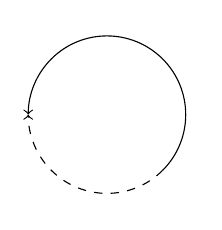
\begin{tikzpicture}
\tzhelplines(4,3)
\tzdots*(1,1)(3,2);
\tzarc [blue,->]   (1,1)(-45:180:1)
\tzarc'[dashed,->] (1,1)(-45:180:1)
\draw [->](3,2) ++(-45:1) arc (-45:180:1);
\draw [dashed,->](3,2) ++(-45:1) arc (-45:180-360:1);
\end{tikzpicture}
\end{tzcode}

You can add text along the arc by specifying the options |{<text>}| and |[<node opt>]| immediately after the two mandatory arguments.


\begin{tzcode}{.3}
% \tzarc('): adding text
\begin{tikzpicture}
\tzhelplines(4,3)
\tzarc [blue,->]  (1,1)(-45:180:1){A}[r]
\tzarc'[dashed,->](1,1)(-45:180:1)
\tzarc[->]        (3,2)(-45:180:1){arc}[midway,sloped]
\tzarc'[dashed,->](3,2)(-45:180:1)
\end{tikzpicture}
\end{tzcode}

You can move arcs by specifying the option |<shift coor>| before the center coordinate or immediately before the option |"<path name>"| if it exists.
The \xem{empty} shift option |<>| is \xem{not allowed}.

\begin{tzcode}{.3}
% \tzarc('): shift, name path, intersection
\begin{tikzpicture}
\tzhelplines(4,3)
\tzarc [blue,->]       (1,1)(-45:180:1){A}[r]
\tzarc'[dashed,->]     (1,1)(-45:180:1)
\tzarc [blue,->]  <2,1>(1,1)(-45:180:1){A-shifted}[r]
\tzarc'[dashed,->]<2,1>"AA"(1,1)(-45:180:1) %%
\tzvXpointat*{AA}{2.5}
\end{tikzpicture}
\end{tzcode}

You can also extend the path of |\tzarc| by specifying the last option |<code.append>| with \Tikz\ code written in it. For example, |<--cycle>| makes the path closed.


\begin{tzcode}{.3}
% \tzarc('): <code.append>
\begin{tikzpicture}
\tzhelplines(4,3)
\tzarc [blue,->](1,1)(-45:180:1)
  < to[bend left] ++(1,-1) >
\tzarc [red,->]  <2,1>(1,1)(-45:180:1)<--cycle>
\end{tikzpicture}
\end{tzcode}



\subsection{Elliptical arcs}
\label{ss:ellipticalarc}

|\tzarc| draws an \iisw{elliptical arc} if you specify |x-radius| and |y-radius|.

\begin{tzcode}{.3}
% \tzarc: elliptical
\begin{tikzpicture}
\tzhelplines(4,4)
\tzarc[->,red](1,1)(30:270:1.5 and 0.5)
\tzarc'[->,dotted](1,1)(30:270:1.5 and 0.5)
\tzdots*(1,1)(2,2);
\tzarc[->,blue,dashed](2,2)(0:-270:1 and 2)
\tzarc'[->](2,2)(0:-270:1 and 2)
\end{tikzpicture}
\end{tzcode}


\begin{tzcode}{.3}
% \tzarc: elliptical
\begin{tikzpicture}
\tzhelplines(4,4)
\tzarc[->,red](1,1)(30:270:1.5 and 0.5)
\tzdots*(1,1)(2,2);
\tzarc[blue,fill=green,fill opacity=.3]
  (2,2)(0:-270:1 and 2)<--(2,2)--cycle> % code.append
\tzarc[->,blue,dashed]
  <1,0>(2,2)(0:-270:1 and 2) % shift
\end{tikzpicture}
\end{tzcode}




%%------------------------------------------------------------
\section{\protect\cmd{\tzarcfrom(')}: Arcs as in \Tikz}
\label{s:tzarcfrom}

\icmd{\tzarcfrom} draws an arc starting from a specified point, like \Tikz\ does.

\begin{tzdef}
% syntax: minimum
\tzarcfrom(<coor>)(<angA:angB:radius>)
% syntax: full
\tzarcfrom[<opt>]<shift coor>"<path name>"
      (<coor>)(<angA:angB:radius>){<text>}[<node opt>]<code.append>
% defaults
  []<>""(<m>)(<m>){}[]<>
\end{tzdef}


\begin{tztikz}
\tzarcfrom(1,1)(30:120:1) % works like:
  \draw (1,1) arc (30:120:1);
\end{tztikz}

\xem{Everything else is the same as in }|\tzarc|.

\icmd{\tzarcfrom'} is the \iisw{swap version} of |\tzarcfrom|.


\begin{tzcode}{.3}
% \tzarcfrom
\begin{tikzpicture}
\tzhelplines(4,3)
\tzdots*(1,1)(3,2);
\tzarcfrom [blue,->]  (1,1)(-45:180:1){A}[r]
\tzarcfrom'[dashed,->](1,1)(-45:180:1)
\tzarcfrom[->](3,2)(-45:180:1){arc}[midway,sloped]
\tzarcfrom'[dashed,->](3,2)(-45:180:1)
\end{tikzpicture}
\end{tzcode}



%%------------------------------------------------------------
\section{\protect\cmd{\tzarcsfrom}: Connected arcs: Semicolon version}
\label{s:tzarcsfrom}

The macro \icmd{\tzarcsfrom} (i.e. |\tzarcs + from|) accepts an arbitrary number of parenthesis arguments in the form of |(<angA:AngB:radius>)| following the start coordinate. Since |tzarcsfrom| is a semicolon version, you need to enter a \xem{semicolon} to indicate when the repetition ends.

\begin{tzdef}
% syntax: minimum
\tzarcsfrom(<start coor>)
           (<angA:angB:radius>)..repeated..(<angA:angB:radius>) ; 
% syntax: full
\tzarcsfrom[<opt>]<shift coor>"<path name>"
           (<start coor>)(<angA:angB:radius>){<text>}[<node opt>]
                         ..repeated..(){}[] ; <code.append>
% defaults
  []<>""(<m>) (<m>){}[]..repeated..(){}[] ; <>
\end{tzdef}


\begin{tzcode}{.4}
% \tzarcfrom: adding text, <code.append>
\begin{tikzpicture}
\tzhelplines(4,4)
\tzcoor*(3,2)(A)
\tzarcsfrom[->,auto](A)
      (0:180:1){1}[midway]
      (180:360:1.2){2}[midway]
      (0:180:1.4){3}[midway,swap]
      (180:360:1.6){4}[midway,swap];
      < node [right,blue] {End!} >
\end{tikzpicture}
\end{tzcode}



\begin{tzcode}{.4}
% \tzarcfrom: shift
% flag: step 1
\begin{tikzpicture}
\tzhelplines(-2,-2)(2,2)
\tzdot*(0,0)
\edef\x{atan(2/3)}
\tzarcsfrom[red,->](0,0)
      (-\x:-\x-180:1){red 1}[midway];
\tzarcsfrom[blue,->](0,0)
      (180-\x:-\x:1){blue 1}[midway];
\tzarcsfrom[dashed,->]<.5,.5>(0,0)
      (180-\x:-\x:1){blue 1}[midway];
\end{tikzpicture}
\end{tzcode}


\begin{tzcode}{.4}
% flag: step 2
\begin{tikzpicture}
\edef\x{atan(2/3)}
\tzarcsfrom[red](0,0)
      (-\x:-\x-180:1){1}[midway]
      (-\x+180:-\x:2){2}[midway]; 
\tzarcsfrom[blue](0,0)
      (180-\x:-\x:1){1}[midway]
      (-\x:-\x-180:2){2}[midway];
\end{tikzpicture}
\end{tzcode}


\begin{tzcode}{.4}
% flag: step 3
\definecolor{flagred}{RGB}{205,48,57}
\definecolor{flagblue}{RGB}{17,73,156}
\begin{tikzpicture}[scale=1]
\edef\x{atan(2/3)}
\tzarcsfrom[draw=none,fill=flagred](0,0)
      (-\x:-\x-180:1)
      (-\x+180:-\x:2) 
      (-\x:-\x+180:1);<-- cycle>
\tzarcsfrom[draw=none,fill=flagblue](0,0)
      (180-\x:-\x:1) 
      (-\x:-\x-180:2) 
      (-\x+180:-\x+360:1);<-- cycle>
\end{tikzpicture}
\end{tzcode}


\begin{tzcode}{.4}
% flag: shift
\definecolor{flagred}{RGB}{205,48,57}
\definecolor{flagblue}{RGB}{17,73,156}
\begin{tikzpicture}[scale=1]
\edef\x{atan(2/3)}
\tzarcsfrom[draw=none,fill=flagred]<.1,.3>(0,0)
      (-\x:-\x-180:1)
      (-\x+180:-\x:2) 
      (-\x:-\x+180:1);<-- cycle>
\tzarcsfrom[draw=none,fill=flagblue](0,0)
      (180-\x:-\x:1) 
      (-\x:-\x-180:2) 
      (-\x+180:-\x+360:1);<-- cycle>
\end{tikzpicture}
\end{tzcode}



%%------------------------------------------------------------
\section{Wedges}
\label{s:wedges}

\subsection{\protect\cmd{\tzwedge(')}}
\label{ss:tzwedge}

\icmd{\tzwedge} draws a wedge around a specified \xem{center} coordinate.

|\tzwedge| works similarly to |\tzarc|, but it forms a closed path from the center coordinate. |\tzwedge| does not have the option |<code.append>|.

\begin{tzdef}
% syntax
\tzwedge[<opt>]<shift coor>"<path name>"
        (<coor>)(<angA:angB:radius>){<text>}[<node opt>]
% defaults
  []<>""(<m>)(<m>){}[midway]
\end{tzdef}


\begin{tztikz}
\tzwedge(1,1)(30:120:1) % works like:
  \draw (1,1) -- ++(30:1) arc (30:120:1) -- cycle;
\end{tztikz}

The swap version \icmd{\tzwedge'} is the \iisw{swap version} of \icmd{\tzwedge}.
It switches the drawing direction from \ixxw{counterclockwise} to \ixxw{clockwise} and vice versa.


\begin{tztikz}
\tzwedge'(1,1)(30:120:1) % works like:
  \draw (1,1) -- ++(30:1) arc (30:120-360:1) -- cycle;
\end{tztikz}

\begin{tzcode}{.3}
% \tzwedge, \tzwedge'
\begin{tikzpicture}
\tzcoor*(2,1)(A)(3pt)
\tzhelplines(4,3)
\tzwedge[blue,very thick](A)(30:120:1.5)
\tzarc[->,green]         (A)(30:120:1.3)
\tzwedge'[dashed](A)(0:135:1.5){clockwise}[sloped,red]
\tzarc'[->,green](A)(0:135:1.3)
\tzwedge'[fill](A)(-60:240:1)
\end{tikzpicture}
\end{tzcode}

\begin{tzcode}{.3}
% \tzwedge('): shift
\begin{tikzpicture}
\tzcoor*(2,1)(A)
\tzhelplines(4,3)
\tzwedge[blue,very thick]<.1,.1>(A)(30:120:1.5) % shift
\tzarc[->,lightgray]<.1,.1>(A)(30:120:1.3)      % shift
\tzwedge'[dashed](A)(0:135:1.5){clockwise}[sloped,red]
\tzarc'[->,lightgray](A)(0:135:1.3)
\tzwedge'[fill]<2,0>(A)(-60:240:1)              % shift
\end{tikzpicture}
\end{tzcode}





\subsection{\protect\cmd{\tzwedge*(')}}
\label{ss:tzwedge*}

The starred version \icmd{\tzwedge*} fills the wedges with |fill=black!50| with |fill opacity=.3| and |text opacity=1|, by default.
With |\settzfillcolor| and |\settzfillopacity|, you can change the default values.
You can also change the fill opacity by specifying the last optional argument |{<fill opacity>}|.

\begin{tzdef}
% syntax:
\tzwedge*[<opt>]<shift coor>"<path name>"
         (<coor>)(<angA:angB:radius>){<text>}[<node opt>]{<fill opacity>}
% defaults:
 *[fill=black!50,fill opacity=.3,text opacity=1]<>""(<m>)(<m>){}[midway]{.3}
\end{tzdef}

\icmd{\tzwedge*'} is the \iisw{swap version} of |\tzwedge*|.

\begin{tzcode}{.3}
% \tzwedge*, \tzwedge*'
\begin{tikzpicture}[->,>=stealth]
\tzhelplines(3,3)
\tzwedge[very thick,blue](1,1)(30:120:1.5)
\tzwedge*[-,very thick,blue,fill=red](1,1)(30:120:1)
\tzwedge'[dashed](1,1)(30:120:1.5){clockwise}[pos=.45]
\tzwedge*'[dashed,fill=green](1,1)(-90:180:1)
\tzdot*(1,1)
\end{tikzpicture}
\end{tzcode}

\begin{tzcode}{.3}
% \tzwedge*('): shift, fill opacity
\begin{tikzpicture}
\tzdot*(1,1)
\tzhelplines(3,3)
\tzwedge[blue,very thick](1,1)(30:120:1.5)
\tzwedge[red,very thick]<.5,.5>(1,1)(30:120:1.5)
\tzwedge'[dashed](1,1)(0:135:1.5)
\tzwedge*[fill=blue](1,1)(300:240:1){B}[b]
\tzwedge*[blue]<2,0>(1,1)(300:240:1){B}[b]{.7}
\end{tikzpicture}
\end{tzcode}

\begin{tzcode}{.3}
% \tzwedge*('): name path, intersections
\begin{tikzpicture}
\tzhelplines(3,3)
\tzwedge'[blue]"AA"(0,1)(45:330:2)
\tzvXpointat{AA}{1}(A)
\tzdots*(A){A}[al](A-2);
\tzwedge*'[blue,fill=red]
         (0,1)(45:330:2mm){$\theta$}[midway,r]
\end{tikzpicture}
\end{tzcode}




%%------------------------------------------------------------
\section{Angle marks}
\label{s:anglemarks}


%%------------------------------------------------------------
\subsection{\protect\cmd{\tzpointangle}: Angles between points}
\label{ss:tzpointangle}

\icmd{\tzpointangle}|(<coor1>)(<coor2>)(<\mymacro>)| computes the angle between two points and allows you to use, where |(coor1)| serves as the coordinate of the center.

\begin{tzcode}{.3}
\begin{tikzpicture}[font=\scriptsize]
\tzhelplines(5,4)
\tzcoors*(4,2)(A){A}(1,1)(B){B}[135];
\tzline[red,dashed](0,1)(5,1)
\tzline[tzextend={1cm}{1cm}](B)(A) % (B): center
\tzpointangle(B)(A){\myAngA}
\tznode(3,1){\myAngA\textdegree}[ar=2mm,absolute]
\tzarc(1,1)(0:\myAngA:2cm)
\end{tikzpicture}
\end{tzcode}



\begin{tzcode}{.3}
\begin{tikzpicture}[font=\scriptsize]
\tzhelplines(5,4)
\tzcoors*(4,2)(A){A}(1,1)(B){B}[135](2,3)(C){C} ;
\tzline[red,dashed](0,1)(5,1)
\tzline[tzextend={1cm}{1cm}](B)(A)
\tzline[tzextend={1cm}{1cm}](B)(C)
\tzpointangle(B)(A){\myAngA}
\tznode(3,1){\myAngA\textdegree}[ar=2mm,absolute]
\tzarc(1,1)(0:\myAngA:2cm)
\tzpointangle(B)(C){\myAngC}
\tznode(2,2){\myAngC\textdegree}[r=3mm]
\tzarc(1,1)(0:\myAngC:1.5cm)
\tzarc(1,1)(\myAngA:\myAngC:10pt){$\theta$}[ar,midway]
\tzarc(1,1)(\myAngA:\myAngC:11pt)
\end{tikzpicture}
\end{tzcode}


\begin{tzcode}{.3}
\begin{tikzpicture}[font=\scriptsize]
\tzhelplines(5,4)
\tzcoors*(4,2)(A){A}(1,1)(B){B}[135](2,3)(C){C} ;
\tzline[tzextend={1cm}{1cm}](B)(A)
\tzline[tzextend={1cm}{1cm}](B)(C)
\tzpointangle(B)(A){\myAngA}
\tzpointangle(B)(C){\myAngC}
\tzarc(1,1)(\myAngA:\myAngC:10pt){$\theta$}[ar,midway]
\tzarc(1,1)(\myAngA:\myAngC:11pt)
\end{tikzpicture}
\end{tzcode}


%%------------------------------------------------------------
\subsection{\protect\cmd{\tzanglemark(')}: Angle marks}
\label{ss:tzanglemark}

\icmd{\tzanglemark} accepts three mandatory coordinates to display an angle mark by an arc (of radius |10pt|, by default) for the second coordinate, on the |behind| layer by default.
You can change the angle arc radius by \icmd{\settzAAradius}.
You can change the layer by \icmd{\settzanglelayer}. Its alias is |\settzanglemarklayer|.

The default line width of angle marks is |very thin|. You can change the default line with with \icmd{\settzAAlinestyle}.

\begin{tzdef}
% syntax: minimum
\tzanglemark(<coorA>)(<coorB>)(<coorC>)
% syntax: full
\tzanglemark[<opt>](<coorA>)(<coorB>)(<coorC>){<text>}[<node opt>](<arc radius>)
% defaults
  [very thin](<m>)(<m>)(<m>){}[pos=1.5](10pt)
\end{tzdef}

You can add angle text by the options |{<text>}| and |[<node opt>]|.

\begin{tzcode}{.3}
% simple example
\begin{tikzpicture}
\tzcoors*(4,2)(A){A}(1,1)(B){B}[180](2,3)(C){C} ;
\tzlines(A)(B)(C);
\tzanglemark(A)(B)(C){$\theta$} % angle mark
\end{tikzpicture}
\end{tzcode}

\begin{tzcode}{.3}
% \settzAAradius
\begin{tikzpicture}
\tzcoors(4,2)(A){A}(1,1)(B){B}[180](2,3)(C){C} ;
\tzlines(A)(B)(C);
\tzlines[thick,blue](A)(2.5,0)(C);
\tzanglemark(A)(B)(C){$\theta$}             %%
\settzAAradius{20pt}                        %%
\tzanglemark(C)(2.5,0)(A){$\alpha$}[pos=.7] %%
\end{tikzpicture}
\end{tzcode}


\paragraph{How it works} Every |\tzanglemark| calculates angles (from 0\textdegree to 360\textdegree) and stores the values under the names \icmd{\tzangleONE} and \icmd{\tzangleTWO}. The difference of the two numbers is stored as an absolute value under the name \icmd{\tzangleresult}.
Of course, you can use these values \xem{only after} running |\tzanglemark|.
\begin{itemize}\firmlist
\item |\tzanglemark| draws an angle mark between two angles, |counterclockwise|, from small two large.
\item |\tzanglemark'| draws an angle mark between two angles, |clockwise|, from small to large.
\end{itemize}

\begin{tzcode}{.3}
\begin{tikzpicture}
\tzhelplines(4,3)
\tzcoors*(4,2)(A){A}(1,1)(B){B}[180](2,3)(C){C} ;
\tzlines(A)(B)(C);
\tzanglemark[->](A)(B)(C){$\theta$}
\tznode[scale=.7](3,1){ONE: \tzangleONE}[r]
\tznode[scale=.7](3,.5){TWO: \tzangleTWO}[r]
\tznode[scale=.7](3,0){$\theta$: \tzangleresult}[r]
\end{tikzpicture}
\end{tzcode}


\remark Simple to use:
\begin{itemize}\firmlist
\item
|\tzmarkanlge(A)(B)(C)| draws an angle mark by an arc from |(A)| to |(C)| about |(B)|.
\item
|\tzmarkanlge(C)(B)(A)| draws an angle mark by an arc from |(C)| to |(A)| about |(B)|.
\item Ignoring the direction, |\tzanglemark(A)(B)(C)| and |\tzanglemark(C)(B)(A)| give the same result.
\end{itemize}

\begin{tzcode}{.3}
\begin{tikzpicture}
\tzhelplines(4,3)
\tzcoors*(4,2)(A){A}(1,1)(B){B}[180](2,3)(C){C} ;
\tzlines(A)(B)(C);
\tzanglemark[->](C)(B)(A){$\theta$}
\tznode[scale=.7](3,1){ONE: \tzangleONE}[r]
\tznode[scale=.7](3,.5){TWO: \tzangleTWO}[r]
\tznode[scale=.7](3,0){$\theta$: \tzangleresult}[r]
\end{tikzpicture}
\end{tzcode}

\paragraph{Swap version}
The \iisw{swap version} \icmd{\tzanglemark'} draws an angle mark for an angle in $360\text{\textdegree}-\theta$.
In other words, |\tzanglemark'| \xem{switches the direction} of drawing an angle arc from |counterclockwise| to |clockwise|, and vice versa.

\begin{tzcode}{.3}
\begin{tikzpicture}
\tzhelplines(4,3)
\tzcoors*(4,3)(A){A}(1,2)(B)(3,0)(C){C}[0] ;
\tzlines[thick](A)(B)(C);
\tzanglemark[->](A)(B)(C){$\theta$}
\tznode[scale=.7](3,2){ONE: \tzangleONE}[r]
\tznode[scale=.7](3,1.5){TWO: \tzangleTWO}[r]
\tznode[scale=.7](3,1){$\theta$: \tzangleresult}[r]
\tzanglemark'[->](A)(B)(C){$\theta'$}(15pt) % swap
\end{tikzpicture}
\end{tzcode}



\paragraph{Angle mark text position}
The midpoint of an angle arc is stored under the coordinate name |tzAAmid|.
The angle mark text is put on the line that goes through the middle point and \icmd{(tzAAmid)}. The default |(<arc radius>)| is |10pt| and the default position of angle text is |pos=1.5| in |[<node opt>]|.

\begin{tzcode}{.3}
% angle marc text position
\begin{tikzpicture}
\tzhelplines(4,3)
\tzcoors*(4,2)(A){A}(1,1)(B){B}[180](2,3)(C){C} ;
\tzlines(A)(B)(C);
\tzanglemark(C)(B)(A){$\theta$}[pos=.65](20pt) %%
\tzdot*(tzAAmid)
\tzline[red,dashed,tzextend={1cm}{2cm}](B)(tzAAmid)
\end{tikzpicture}
\end{tzcode}

\remark Instead of using the options |{<text>}| and |[<node opt>]|, you can also use the coordinate |(tzAAmid)| to place the angle text wherever you want, without using |\tzanglemark(')|. Of course, you can use the correct |(tzAAmid)| only after running |\tzanglemark|.



%%------------------------------------------------------------
\subsection{\protect\cmd{\tzanglemark*(')}: Fill angle marks}
\label{ss:tzanglemark*}

\icmd{\tzanglemark*} fills (in the |behind| layer, by default) the angle mark area with |fill=black!50| and with the options |fill opacity=.3| and |text opacity=1| by default. It does not draw any lines: |[draw=none]| by default.

Using the macros such as |\settzfillcolor|, |\settzfillopacity|, and \icmd{\settzanglelayer}, you can change the default values.



\begin{tzdef}
% syntax: minimum
\tzanglemark*(<coorA>)(<coorB>)(<coorC>)
% syntax: full
\tzanglemark[<opt>](<coorA>)(<coorB>)(<coorC>){<text>}[<node opt>](<arc radius>)
% defaults
  [very thin](<m>)(<m>)(<m>){}[pos=1.5](10pt)
% syntax
\tzanglemark*[<opt>](<coor1>)(<coor2>)(<coor3>)
             {<text>}[<node opt>](<arc radius>){<fill opacity>}
% defaults
  *[very thin,draw=none,fill=black!50,fill opacity=.3,text opacity=1]
   (<m>)(<m>)(<m>){}[pos=1.5](10pt){.3}
\end{tzdef}


\begin{tzcode}{.3}
% \tzanglemark*
\begin{tikzpicture}
\tzhelplines(4,3)
\tzcoors*(4,2)(A){A}(1,1)(B){B}[180](2,3)(C){C} ;
\tzlines(A)(B)(C);
\tzanglemark*[red](C)(B)(A){$\theta$}
\end{tikzpicture}
\end{tzcode}


\icmd{\tzanglemark*'} is the \iisw{swap version} of |\tzanglemark*|.

\begin{tzcode}{.3}
% \tzanglemark*(')
\begin{tikzpicture}
\tzhelplines(4,3)
\tzcoors*(4,3)(A){A}(1,2)(B)(3,0)(C){C}[0] ;
\tzlines(A)(B)(C);
\tzanglemark*[red](A)(B)(C){$\theta$}
\tzanglemark*'[blue](A)(B)(C){$\theta'$}(15pt) % swap
\end{tikzpicture}
\end{tzcode}

\begin{tzcode}{.3}
% \tzanglemark*('): \settzAAlinestyle
\begin{tikzpicture}
\settzAAlinestyle{thick}
\tzhelplines(4,3)
\tzcoors*(4,3)(A){A}(1,2)(B)(3,0)(C){C}[0] ;
\tzlines[thick,blue](A)(B)(C);
\tzanglemark*[red](A)(B)(C){$\theta$}
\tzanglemark(A)(B)(C)
\settzAAlinestyle{very thin} % default
\tzanglemark'(A)(B)(C)(14pt)
\tzanglemark'(C)(B)(A)(15pt){$\theta'$}
\end{tikzpicture}
\end{tzcode}



%%%% (REMOVED!!!)
%%%%%------------------------------------------------------------
%%%\section{\protect\cmd{\tzpicangle}: angle marks}
%%%\label{s:tzpicangle}
%%%
%%%\begin{tzdef}
%%%% syntax: angle ABC or angle CBA
%%%\tzpicangle(')[<angle pic opt>][<path/draw opt>](<coor1>)(<coor2>)(<coor3>)
%%%           {<angle pic text>}[<text eccentricity>](<angle pic arc radius>)
%%%% defaults:(')[][]()()(){}[1.5](10pt)
%%%\end{tzdef}
%%%
%%%When |(coor1) -- (coor2) -- (coor3)| is arranged naturally (counterclockwise),
%%%|\tzarc| draws an arc naturally (counterclockwise), while |tzarc'| draws an arc clockwise.
%%%
%%%When |(coor1) -- (coor2) -- (coor3)| is arranged clockwise,
%%%|\tzarc| draws an arc counterclockwise, while |tzarc'| draws an arc counterclockwise.
%%%
%%%\remark
%%%Internally, |\tzpicangle| is defined to draw an arc by a |pic| operation of \TikZ, so it is not affected by scaling, unless |transform shape| is not used.
%%%
%%%\begin{tzcode}{.3}
%%%\begin{tikzpicture}
%%%\tzhelplines(4,2)
%%%\tzlines(2,2)(1,1)(3,0);
%%%\tzpicangle[->,draw=red,fill=red!30](2,2)(1,1)(3,0){a}
%%%\tzlines     [xshift=1cm](2,2)(1,1)(3,0);
%%%\tzpicangle'[->][xshift=1cm](2,2)(1,1)(3,0){a}
%%%\end{tikzpicture}
%%%\end{tzcode}
%%%
%%%
%%%\begin{tzcode}{.3}
%%%\begin{tikzpicture}
%%%\tzhelplines(4,2)
%%%\tzlines(3,0)(1,1)(2,2);
%%%\tzpicangle[->,fill=red!30](3,0)(1,1)(2,2){a}
%%%\tzlines     [xshift=1cm](3,0)(1,1)(2,2);
%%%\tzpicangle'[->][xshift=1cm](2,2)(1,1)(3,0){a}[.5](1cm)
%%%\end{tikzpicture}
%%%\end{tzcode}
%%%
%%%
%%%\begin{tzcode}{.3}
%%%\begin{tikzpicture}
%%%\tzhelplines(4,2)
%%%\tzlines(2,0)(0,0)(0,2);
%%%\tzpicangle[fill=red!30](2,0)(0,0)(0,2){a}
%%%\tzlines     [xshift=1cm](2,2)(1,1)(3,0);
%%%\tzpicangle'[->][xshift=1cm](2,2)(1,1)(3,0){a}[.5](1cm)
%%%\end{tikzpicture}
%%%\end{tzcode}
%%%
%%%
%%%\begin{tzcode}{.3}
%%%\begin{tikzpicture}
%%%\tzhelplines(4,2)
%%%\tzpicangle  [fill=red!30](2,2)(1,1)(3,0){a}
%%%\tzpicangle'[][xshift=1cm](2,2)(1,1)(3,0){a}
%%%\end{tikzpicture}
%%%\end{tzcode}
%%%
%%%
%%%\begin{tzcode}{.3}
%%%\begin{tikzpicture}
%%%\tzhelplines(4,2)
%%%\tzpicangle    [fill=red!30](3,0)(1,1)(2,2){a}
%%%\tzpicangle'[->][xshift=1cm](2,2)(1,1)(3,0){a}[.5](1cm)
%%%\end{tikzpicture}
%%%\end{tzcode}
%%%
%%%
%%%\begin{tzcode}{.3}
%%%\begin{tikzpicture}
%%%\tzhelplines(4,2)
%%%\tzpicangle    [fill=red!30](2,0)(0,0)(0,2){a}
%%%\tzpicangle'[->][xshift=1cm](2,2)(1,1)(3,0){a}[.5](1cm)
%%%\end{tikzpicture}
%%%\end{tzcode}
%%%
%%%\begin{tzcode}{.3}
%%%\begin{tikzpicture}[scale=.5]
%%%\tzhelplines(4,2)
%%%\tzpicangle    [fill=red!30](2,0)(0,0)(0,2){a}
%%%\tzpicangle'[->][xshift=1cm](2,2)(1,1)(3,0){a}[.5](1cm)
%%%\end{tikzpicture}
%%%\end{tzcode}




\subsection{\protect\cmd{\tzrightanglemark}: Right angle marks}
\label{ss:tzrightangle}

\icmd{\tzrightanglemark} takes three coordinates as mandatory arguments to display a right angle mark for the second coordinate. The mark is drawn on the |behind| layer by default, which can be changed by \icmd{\settzanglelayer}.

The default line with is |very thin|, which can be changed by the option |[<opt>]|. You can also change the line width using \icmd{\settzRAlinestyle}, which is valid until the end of |tikzpicture| environment.
|\settzRAlinestyle| is an alias of |\settzAAlinestyle|.
The length of the side is |5pt| by default, and it can be changed by the last option |(<size>)|.
You can also change the size with \icmd{\settzRAsize}, which is valid until the end of the |tikzpicture| environment.

\begin{tzdef}
% syntax: minimum
\tzrightanglemark(<coorA>)(<coorB>)(<coorC>)
% syntax: full
\tzrightanglemark[<opt>](<coorA>)(<coorB>)(<coorC>){<text>}[<node opt>](<size>)
% defaults
 [very thin](<m>)(<m>)(<m>){}[](5pt)
\end{tzdef}

\begin{tzcode}{.3}
% simple example (with angle text)
\begin{tikzpicture}[font=\scriptsize]
\tzhelplines(4,3)
\tzcoors(1,2)(A){A}(1,0)(B){B}[180](4,0)(C){C}[0];
\tzlines(A)(B)(C);
\tzrightanglemark(A)(B)(C){90\textdegree}
\end{tikzpicture}
\end{tzcode}

\remark 
\begin{itemize}\firmlist
\item |\tzrightanglemark(A)(B)(C)| and |\tzrightanglemark(C)(B)(A)| give the same result.
\item |\tzrightanglemark'| is redundant, but it is provided to avoid frequent coding errors.
\end{itemize} 

Each |\tzrightanglemark| defines \icmd{(tzRAvertex)} as the coordinate of the right angle mark vertex.
The angle text is placed on the line going through the second coordinate and |(tzRAvertex)|. The default position is |pos=2| in |[<node opt>]|.

\begin{tzcode}{.3}
% \settzRAsize
\begin{tikzpicture}
\tzhelplines(4,3)
\tzcoors(2,3)(A){A}(1,1)(B){B}[180](3,0)(C){C}[0];
\tzlines(A)(B)(C);
\settzRAsize{15pt}
\tzrightanglemark(A)(B)(C){90\textdegree}[pos=1.7]
\tzdot*(tzRAvertex)
\tzline[red,dashed,tzextend={2mm}{2cm}](B)(tzRAvertex)
\end{tikzpicture}
\end{tzcode}

\remark You can also use the coordinate |(tzRAvertex)| to place angle text wherever you want, after |\tzrightanglemark|.




\subsection{\protect\cmd{\tzrightanglemark*}: Fill right angle marks}
\label{ss:tzrightangle*}

The starred version \icmd{\tzrightanglemark*} fills the interior of right angle marks with |fill=black!50|, with |fill opacity=.3| and |text opacity=1|. It does not draw any line: |[draw=none]| by default. The filled mark is drawn on the |behind| layer by default, which can be changed by \icmd{\settzanglelayer}.
Its alias is \icmd{\settzanglemarklayer}.

\begin{tzdef}
% syntax: minimum
\tzrightanglemark*(<coorA>)(<coorB>)(<coorC>)
% syntax: full
\tzrightanglemark*[<opt>](<coorA>)(<coorB>)(<coorC>)
                  {<text>}[<node opt>](<size>){<fill opacity>}
% defaults
 *[draw=none,very thin,fill=black!50,fill opacity=.3,text opacity=1]
  (<m>)(<m>)(<m>){}[](5pt){.3}
\end{tzdef}

With \icmd{\settzfillcolor} and \icmd{\settzfillopacity}, you can also change the default fill color and fill opacity.


\begin{tzcode}{.3}
% \rightanglemark*
\begin{tikzpicture}[scale=.8,font=\scriptsize]
\tzhelplines(5,5)
\tzcoorsquick(0,5)(A)(4,0)(B)(0,1)(C)(5,5)(D);
\tzline"AB"(A)(B)
\tzline"CD"(C)(D)
\tzXpoint{AB}{CD}(E)
\tzrightanglemark*(A)(E)(D){90\textdegree}
\tzrightanglemark*[red](A)(E)(C)(20pt)
\tzrightanglemark*[draw=blue,fill=green](B)(E)(C)(20pt)
\end{tikzpicture}
\end{tzcode}


\begin{tzcode}{.3}
% \settzRAsize
\begin{tikzpicture}[scale=.8,font=\scriptsize]
\tzhelplines(5,5)
\tzcoorsquick(0,5)(A)(4,0)(B)(0,1)(C)(5,5)(D);
\tzline[dotted]"AB"(A)(B)
\tzline[dotted]"CD"(C)(D)
\tzXpoint{AB}{CD}(E)
\settzRAsize{20pt} %%
\tzrightanglemark*[red](A)(E)(D){$\rho$}[pos=1.3]
\tzrightanglemark[blue,thin](A)(E)(D)
\tzrightanglemark*[draw=blue,thin,fill=green](B)(E)(C)
\end{tikzpicture}
\end{tzcode}


\section{\protect\cmd{\tzdistance}: Distances and changes}
\label{s:tzdistance}

\icmd{\tzdistance}|(<coor1>)(<coor2>){<\mylength>}| calculates the Cartesian distance \xem{from} |(<coor1>)| \xem{to} |(<coor2>)| and stores the (absolute) value to the user-specified macro |\mylength| in centimeters. 
And |\tzdistance| also stores the changes in |x| and |y| to |{<\Deltax>}| and |{<\Deltay>}|, respectively.
Note that the calculated distance is \xem{approximate}.

\begin{tzdef}
% syntax: minimum
\tzdistance(<coorA>)(<coorB>){<\mylength>}
% syntax: full
\tzdistance(<coorA>)(<coorB>){<\mylength>}{<\Deltax>}{<\Deltay>}
% defaults:
  (<m>)(<m>){<m>}{}{}
\end{tzdef}

\begin{tzcode}{.3}
% \tzdistance
\begin{tikzpicture}
\tzhelplines(4,3)
\tzcoors*(0,0)(A)(4,0)(B)(0,3)(C);
\tzdistance(A)(B){\lenA}
\tzdistance(B)(C){\lenB}
\tzpolygon(A){\lenA}[b](B){\lenB}[sloped,a](C);
\end{tikzpicture}
\end{tzcode}

\begin{tzcode}{.3}
% \tzdistance, \tzpointangle
\begin{tikzpicture}
\tzhelplines(4,3)
\tzcoors*(1,0)(A){A}[180](3,1)(B){B}[0];
\tzdistance(A)(B){\lenA}{\xdist}{\ydist}
\tzpointangle(A)(B){\angA}
\tzline[red](A)(B)
\tzarc[blue](A)(\angA:90:\lenA)
\tzline+[<->]<0,-.5>(A)(\xdist,0)
\tzline+[<->]<1,0>(A-|B)(0,\ydist)
\end{tikzpicture}
\end{tzcode}

\begin{tzcode}{.3}
% \Deltax: (+), \Deltay: (-)
\begin{tikzpicture}
\tzhelplines(4,3)
\tzcoors*(1,2)(A){A}[180](3,1)(B){B}[0];
\tzdistance(A)(B){\lenA}{\xdist}{\ydist}  % A to B
\tzpointangle(A)(B){\angA}
\tzline[red](A)(B)
\tzarc[->,blue](A)(\angA:90:\lenA)
\tzline+[|->|]<0,-.5>(A|-B)
                     {$\Delta\,x=\xdist$}[b]
                     (\xdist,0)
\tzline+[|->|]<-1,0>(A)(0,\ydist)
\end{tikzpicture}
\end{tzcode}


\begin{tzcode}{.3}
% \Deltax: (-), \Deltay: (+)
\begin{tikzpicture}
\tzhelplines(4,3)
\tzcoors*(1,2)(A){A}[180](3,1)(B){B}[0];
\tzdistance(B)(A){\lenA}{\xdist}{\ydist}  % B to A
\tzpointangle(B)(A){\angA}
\tzline[red](B)(A)
\tzarc'[->,blue](A)(\angA-180:90:\lenA)
\tzline+[|->|]<0,-.5>(B)
                     {$\Delta\,x=\xdist$}[b]
                     (\xdist,0)
\tzline+[|->|]<-1,0>(B-|A)(0,\ydist)
\end{tikzpicture}
\end{tzcode}


